\documentclass{ansnse}
\usepackage{authblk}
\usepackage{amsmath}
\usepackage{siunitx}
\usepackage{isotope}
\usepackage[margin=1in]{geometry}
\usepackage{setspace}
\usepackage{verbatim}
\usepackage{graphicx}
\usepackage{todonotes}
\usepackage{subfig}
\usepackage{booktabs}
\usepackage{multirow}

\usepackage{hyperref}
\hypersetup{colorlinks=true,
citecolor=black,
linkcolor=black}

\sisetup{list-final-separator={, and },
separate-uncertainty=true,
range-phrase={--},
multi-part-units=single,
list-units=single,
range-units=single}

\widowpenalty=1000
\clubpenalty=1000

\author{Jeremy Lloyd Conlin\footnote{\texttt{jlconlin@lanl.gov}} }  % PNAR, MC
\author{Stephen J. Tobin}   % Overall effort
\author{Adrienne M. LaFleur}    % SINRD
\author{Jianwei Hu}         % CIPN
\author{TaeHoon Lee}        % DDA
\author{Nathan P. Sandoval} % DN
\author{Melissa A. Schear}  % DDSI

\affil{\normalsize\emph{Los Alamos National Laboratory,
Los Alamos, NM 87544}}

\title{On Using Code Emulators and Monte Carlo Estimation to Predict Assembly Attributes of Spent Fuel Assemblies for Safeguards Applications}

\date{}

\DeclareMathAlphabet{\mathpzc}{OT1}{pzc}{m}{it}

\newcommand{\PuEff}{\ensuremath{\isotope[239]{Pu}_{\text{e}}}}
\newcommand{\Pub}{\ensuremath{\PuEff'}}
\newcommand{\dd}{\ensuremath{\mathop{}\!\mathrm{d}}}
\newcommand{\weight}{\ensuremath{\mathpzc{w}}}

\begin{document}
\maketitle
%\ansabstract{The quantification of the plutonium mass in spent nuclear fuel assemblies is an important measurement for nuclear safeguards practitioners.  A program is well underway to develop nondestructive assay instruments which, when combined, will be able to quantify the plutonium content of a spent nuclear fuel assembly.  Each instrument will quantify a specific attribute of the spent fuel assembly e.g., the fissile content.  In this paper, we present a Monte Carlo-based method of estimating the mean and distribution of some assembly attributes.  An MCNPX model of each instrument has been created and the response of the instrument was simulated for a range of spent fuel assemblies with discrete parameters (e.g., burnup, initial enrichment, and cooling time).  The Monte Carlo-based method interpolates between the modeled results for an instrument to emulate a response for parameters not explicitly modeled.  We demonstrate the usefulness of this technique in applying the technique to six different instruments under investigation. The results show that this Monte Carlo-based method can be used to estimate the assembly attributes of a spent fuel assembly based upon the measured response from the instrument.
%}
keywords: Monte Carlo, emulation, safeguards.
  \doublespacing

\section{Introduction}\label{sec:Introduction}
Quantifying the plutonium mass in spent nuclear fuel assemblies is a problem of concern to the International Atomic Energy Agency (IAEA).  Ensuring that no nuclear material is maliciously diverted from an assembly requires close monitoring of the spent fuel assemblies after their removal from nuclear reactors around the world. 

The IAEA already monitors spent nuclear fuel reprocessing plants and storage facilities, typically by using cameras and visual inspections.  In addition, gamma and neutron measurements are taken, but the operator's declaration of the parameters (i.e., burnup, initial enrichment, and time since removed from a reactor) are used as a reference to the measurements.  These radiation measurements and visual inspection can't measure the plutonium content of the spent nuclear fuel assembly, they can only
detect some types of changes to the assembly.

Under the sponsorship of the Next Generation Safeguards Initiative (NGSI) an effort is underway \citep{Tobin:2008Deter-0} to measure the plutonium content of spent nuclear fuel assemblies without relying on the operator's declaration of the operating parameters of the nuclear reactor and without previous measurements of the spent nuclear fuel assembly.  This effort is focusing on a variety of non-destructive assay (NDA) techniques that can be used in a variety of surroundings (e.g., air, water, borated water), and are fast enough to not be a burden on the operational procedures in a nuclear reactor, spent fuel storage, or reprocessing facility.  A few of these techniques will be integrated into one instrument to allow a safeguards inspector to measure the mass of plutonium in a spent nuclear fuel assembly and determine whether spent fuel pins have been removed from the assembly.

The program to develop a combination of instruments---integrated in such a way as to quantify the mass of plutonium---is, recognizably, a grand challenge.\cite{Veal:2010NGSI--0}  We are currently investigating fourteen different NDA instruments as part of this program.  No single instrument can measure the plutonium mass directly, but each instrument provides a measurement, which contributes a piece of the puzzle necessary to quantify the plutonium mass.  Some of the quantities that can be measured from an individual measurement are: the average burnup of an assembly; the ratio of the mass of the fissile isotopes to the mass of the fertile isotopes (fissile/fertile ratio); the ratio of the mass of elemental uranium to the mass of elemental plutonium (elemental U/Pu ratio); the mass of \isotope[235]{U} to the mass of \isotope[239]{Pu} (\isotope[235]{U}/\isotope[239]{Pu} ratio); and a combination of the masses of the three fissile isotopes, \isotope[235]{U}, \isotope[239]{Pu}, and \isotope[241]{Pu} (fissile content).

In order to determine the response of each of the fourteen NDA techniques to spent nuclear fuel assemblies, we have created an MCNPX\cite{Pelowitz:2009MCNPX-0} model of each instrument.  A library of spent fuel assemblies has been created \cite{Fensin:2009A-Mon-0} which contains a wide variety of spent fuel assemblies.  The models are \mbox{17 x 17}, PWR assemblies with assembly parameters of \SIlist[list-final-separator={, or }]{15; 30; 45; 60}{GWd/tU} burnup; \SIlist[list-final-separator={, or }]{2; 3; 4; 5}{wt \% \isotope[235]{U}} initial enrichment; and \SIlist[list-final-separator={, or }]{1; 5; 20; 80}{yr} cooling time.  The parameters of burnup, initial enrichment, and cooling time define the mass and spatial distribution of the many isotopes in the spent fuel assembly.  

The combination of assembly parameters of burnup, initial enrichment, and cooling time give 64 different models of spent nuclear fuel assemblies which are representative of spent nuclear fuel assemblies in existence in nuclear reprocessing, storage, or reactor sites.  The models are combined with the geometry of the detectors and a fixed source MCNPX calculation is performed with a variety of tallies to estimate the response of the detectors used in the technique.  The detector responses can then be used to estimate the measured quantity of the technique.  The MCNPX simulations can be performed with the assembly surrounded by either water, borated water (2200 ppm), or air.

Each of the fourteen NDA instruments has some detector response that changes with some attribute of the assembly (e.g., fissile content, elemental U/Pu ratio, etc.).  The goal for each instrument is to accurately predict an assembly attribute for a given detector response.  One detector may measure neutrons while the instrument response scales with the fissile content.  Another detector may preferentially measure delayed neutrons that scales with the \isotope[235]{U}/\isotope[239]{Pu} ratio.  Both the fissile content and \isotope[235]{U}/\isotope[239]{Pu} ratio are assembly attributes.  Though an individual MCNPX simulation can estimate the detector response and can estimate or calculate a particular assembly attribute, it can be computationally expensive.  However, a single simulation cannot estimate a \emph{distribution} of assembly attributes for a measured detector response.  Furthermore, one MCNPX simulation estimates the detector response from a single set of parameters defining a spent fuel assembly and there can be many sets of parameters that produce the same detector response.

To illustrate, we show in Figure \ref{fig:Example} a typical detector response vs.\ assembly attribute.  These are the results of simulating one of our instruments using the 64 spent fuel assembly models surrounded by water.  The colors in the figure represent the burnup parameter and the marker shape represents the initial enrichment.  The difference in cooling time is not explicitly shown, but it is known that the cooling time increases as the assembly attribute decreases.  Error bars arising from using a finite number of MCNPX histories are shown in this figure (and in all the figures of this paper) but are smaller than the plot markers.  The statistical uncertainty (the standard deviation of the reproducibility of the MCNPX results) in these calculations is approximately 0.2\% relative to the true value.  If a measurement was made and the detector gave a response of \num{1.600(8)}, there are no fewer than five assemblies that would give the same detector response and each has a different value for the assembly attribute such as \isotope[235]{U} or elemental \isotope{Pu} mass.  As well, there are many additional assemblies not specifically modeled that would have the same detector response, e.g.,\ a spent fuel assembly with \SI{30}{GWd/tU}, \SI{2.5}{wt \% \isotope[235]{U}} initial enrichment, and \SI{5}{yr} cooling time parameters.  We see, therefore, the difficulty in using the measured detector response to predict the assembly attribute for an unknown spent fuel assembly.
\begin{figure}[h]\centering
    \includegraphics[width=0.75\textwidth, keepaspectratio]{Figures/Plain/PNARH2O}
    \caption{Sample data showing detector response scaling with assembly attribute.}
    \label{fig:Example}
\end{figure}

This paper reports a Monte Carlo-based method developed to predict certain assembly attributes from a measured detector response.  The method relies on explicit modeling of the detector response for a variety of spent fuel assemblies for which the assembly attribute is known or can be estimated in the MCNPX simulation.  This Monte Carlo method of estimating assembly attributes from modeled data requires interpolation between the modeled data points and is akin to emulating MCNPX simulations.  In Section \ref{sec:MCEstimate} we discuss the emulation of MCNPX simulations and the interpolation between explicitly simulated results.  We also introduce the Monte Carlo-based method of estimating the assembly attributes.

We present some numerical results in Section \ref{sec:Simulations} for several of the NDA techniques we have simulated to demonstrate the effectiveness of the Monte Carlo method.  Finally in Section \ref{sec:Conclusions} we draw some conclusions and discuss future work.

\section{Code Emulation and Monte Carlo Estimates}\label{sec:MCEstimate}
In each of the instruments being explored as part of the effort to quantify the plutonium content of spent nuclear fuel assemblies, some assembly attribute is desired from some measured detector response.  We only have the detector response (e.g., total neutron count) and we must infer some assembly attribute (e.g., fissile content).  A one-to-one relationship between the detector response and assembly attribute is ideal as the assembly attribute mean and distribution would be known exactly from the measured detector response and its associated uncertainty. 

In dealing with the complexity of spent nuclear fuel, we are not so fortunate as to work with such ideal assemblies.  A spent nuclear fuel assembly has myriad of different isotopes, some are fissile and others have large absorption cross sections.  Each isotope behaves differently as the assembly parameters change.  Nevertheless, it is possible to estimate a mean value and distribution for a particular assembly attribute given a measured detector response.  An example of the complexity in the relationship between the detector response and the assembly attribute is shown in Figure \ref{fig:Example}.  We can see that there are some general trends in the data with regards to burnup, initial enrichment, and cooling time.  However, we do not have a one-to-one relationship between the detector response and the assembly attribute.

\subsection{Interpolation and Code Emulation}\label{sec:InterpolationandEmulation}
The 64 models in our library of spent fuel assembly models span a wide range of burnup, cooling time, and initial enrichment, and encompass most of the spent fuel assemblies expected in spent fuel storage facilities.  Despite the broad range of assemblies modeled, it is in no way a complete set of spent nuclear fuel assemblies.  Reactor operators are free to operate their reactor and burn their fuel to whatever specifications for which the reactor was designed; they are not limited to \SIlist[list-final-separator={, or }]{15; 30; 45; 60}{GWd/tU}.  Similarly, it is unlikely that measurements of a spent fuel assembly will be made at exactly \SIlist[list-final-separator={, or }]{1; 5; 20; 80}{yr} since the assembly was removed from the reactor or that the assembly will initially have had an enrichment of \SIlist[list-final-separator={, or }]{2;3;4;5}{wt \% \isotope[235]{U}}.  

Many of the simulations performed in our investigation of the fourteen NDA techniques require more than 200 CPU hours to reduce the level of statistical uncertainty in our calculations to acceptable values.  This is in addition to computer time required to create the assembly model.  The computational expense of performing such a simulation is too great to be used for every measurement of a spent fuel assembly.  

Instead of running MCNPX for every measured spent fuel assembly, the results of the simulations of the 64 spent fuel assembly models can be interpolated to create functions that map assembly parameters (e.g., burnup, initial enrichment, and cooling time) to the detector response and desired assembly attribute.  Once mapping functions have been created, through interpolation of existing data, new data can be inferred from the mapping functions.  

The idea of using knowledge of a system from previous measurements or simulations with specific parameters to predict a system response at other parameters is not new.  In geostatistics this is known as ``kriging''\cite{Krige:1951A-Sta-0,Matheron:1973The-i-0} and has been used for decades.   In their paper, \citet{Heitmann:2006Cosmi-0} call this code \emph{emulation} as compared to the explicit \emph{simulation} of the system response.  To the best of our knowledge, this is the first time this has been applied to safeguards applications. 

We have chosen to use radial basis functions to perform the interpolation between the 64~spent fuel assembly models and the detector response or assembly attribute.  The interpolating function is a linear function between the data points.  Radial basis functions are well suited for applications\cite{Buhmann:2003Radia-0}
\begin{enumerate}
    \item that depend on many variables or parameters,
    \item that are defined by possibly very many data, and
    \item for which the data are `scattered' in their domain.
\end{enumerate}
We see from Figure \ref{fig:Example} that our data are many, scattered, and depend on many parameters, thus radial basis functions meet the needs for our interpolation.  In addition, radial basis functions are capable of performing interpolations in many dimensions.

For our work, two different, three dimensional, mapping functions are needed
\begin{subequations}
    \label{eq:Maps}
    \begin{align}
        D &= M_{D}(B, E, C) \label{eq:Response} \\
        P &= M_{P}(B, E, C), \label{eq:Attribute}
    \end{align}
\end{subequations}
where $B$, $E$, and $C$ are the burnup, initial enrichment, and cooling time respectively.  Together these three parameters define an assembly model, $A$.  $M_{D}$ is the mapping function from the assembly model to the detector response, $D$, and $M_{P}$ is the mapping function from the assembly model to the assembly attribute $P$.  

\subsection{Monte Carlo Estimate of Assembly Attributes}
With the mapping functions defined, we can estimate the mean and distribution of an assembly attribute via a Monte Carlo-based method given a detector response.  Typically the detector response will be measured by an instrument in the field and the assembly attribute must be inferred from the detector response.  Since none of our NDA techniques have yet been built, all detector responses in this paper are the results of MCNPX simulations.  Regardless of whether the detector response is measured or simulated we refer to it as the \emph{measured} detector response.

The mean assembly attribute can be calculated as
\begin{equation}
    \overline{P} = \int_{\Delta B}\int_{\Delta E}\int_{\Delta C} R(D, \mu, \sigma) M_{P}(B, E, C)f(B,E,C) \dd C \dd E \dd B,
    \label{eq:AttributeIntegral}
\end{equation}
where $\Delta B$, $\Delta E$, and $\Delta C$ are ranges of possible burnup, initial enrichment, and cooling time for the assembly and $M_{P}$ is the mapping function from assembly parameters to the assembly attribute (Eq. \eqref{eq:Attribute}).  $f(B,E,C)$ is a three-dimensional probability density function (PDF) defining the probability of each $B$, $E$, and $C$.  

The function $R\left(D,\mu,\sigma\right)$ in Eq. \eqref{eq:AttributeIntegral} is the response function and is defined to be
\begin{equation}
    R(D, \mu,\sigma) = e^{-\frac{(D-\mu)^{2}}{2\sigma^{2}}},
    \label{eq:ResponseWeight}
\end{equation}
where $\mu, \sigma$ are the measured detector response and its standard deviation, and $D$ comes from Eq. \eqref{eq:Response}.  The response is dependent on the assembly parameters, $B$, $E$, and $C$.  We can see that the response function ranges from 0, when $D$ is infinitely far away from the measured detector response, $\mu$, to 1 when $D = \mu$.  The response function serves to reduce the importance of assemblies with a simulated detector response far from the measured detector response.  

To illustrate why we have included the response function we refer again to Figure \ref{fig:Example} and suppose that our measured response is approximately 1.65.  This measured response could be produced by an assembly with \SI{45}{GWd/tU} burnup, \SI{5}{wt \% \isotope[235]{U}}, and \SI{80}{yr} cooling time (represented by the lowest blue diamond in Figure \ref{fig:Example}), with an approximate assembly attribute value of 6500.    However any of the four assemblies with \SI{15}{GWd/tU} burnup and \SI{3}{wt \% \isotope[235]{U}} (green triangles in Figure \ref{fig:Example}) have a value for the assembly attribute close to 6500.  The response function, $R\left(D, \mu,\sigma\right)$, will have to be smaller for the assemblies with \SI{15}{GWd/tU} burnup than the assemblies with \SI{45}{GWd/tU} and its contribution to $\overline{P}$ is reduced.

The multi-dimensional integral in Eq. \eqref{eq:AttributeIntegral} can be estimated using a simple Monte Carlo integration\cite{Lewis:1993Compu-0},
\begin{equation}
    \hat{P} \approx \frac{1}{N} \sum_{k=1}^N R(D_{k},\mu,\sigma) M_{P}(B_k, E_k, C_k),
    \label{eq:MCAttributeIntegral}
\end{equation}
where $B_{k}$, $E_{k}$, and $C_{k}$ are random samples of burnup, initial enrichment and cooling time that define a randomly sampled spent fuel assembly, $A_{k}$, and $D_{k} = M_{D}(B_{k}, E_{k}, C_{k})$ is the simulated detector response for $A_{k}$.  To calculate the distribution, or probability density function, associated with $\hat{P}$, one can simply bin the individually sampled results and their weights and construct a frequency plot of the assembly attribute.

The values for the assembly parameters $B_{k}$, $E_{k}$, and $C_{k}$, are randomly sampled from the PDF $f(B,E,C)$.  Without additional knowledge, we assume that these values are equally probable throughout the whole range of possible values; i.e., \SIrange{15}{60}{GWd/tU}, \SIrange{2}{5}{wt \% \isotope[235]{U}}, and \SIrange{1}{80}{yr}.  The PDF, $f(B,E,C)$ would be defined as
\begin{equation}
    f_{\Pi} = \Pi_{B}\Pi_{E}\Pi_{C},
    \label{eq:UniformPDF}
\end{equation}
with $\Pi_{X}$ being the uniform PDF of picking parameter $X$ over its appropriate range;
\begin{subequations}
    \label{eq:UniformPi}
    \begin{align}
        \Pi_{B} &= \frac{1}{60-15}, \\
        \Pi_{E} &= \frac{1}{5-2}, \\
        \Pi_{C} &= \frac{1}{80-1}.
    \end{align}
\end{subequations}
Suppose an independent measurement provided information about burnup i.e., \SI{45.00(225)}{GWd/tU} (5\% uncertainty).  Rather than sampling an assembly parameter from the uniform PDFs in Eqs. \eqref{eq:UniformPi}, we can sample from a PDF that uses information about the measured assembly parameter.  Independent measurements of the other assembly parameters can also be included.  With information about all three assembly parameters from independent measurements, our PDF, $f(B,E,C)$ can be defined as
\begin{equation}
    f_{\Lambda} = \Lambda_{B}\Lambda_{E}\Lambda_{C},
    \label{eq:GaussianPDF}
\end{equation}
with $\Lambda_{X}$ being the uniform PDF of picking parameter $X$ over its appropriate range;
\begin{subequations}
    \label{eq:GaussianLambda}
    \begin{align}
        \Lambda_{B} &= \frac{1}{\sqrt{2\pi \left(\sigma_{B}\right)^{2}}} e^{-\frac{\left(B-B_{m}\right)^{2}}{2 \left(\sigma_{B}\right)^{2}}}, \\
        \Lambda_{E} &= \frac{1}{\sqrt{2\pi \left(\sigma_{E}\right)^{2}}} e^{-\frac{\left(E-E_{m}\right)^{2}}{2 \left(\sigma_{E}\right)^{2}}}, \\
        \Lambda_{C} &= \frac{1}{\sqrt{2\pi \left(\sigma_{C}\right)^{2}}} e^{-\frac{\left(C-C_{m}\right)^{2}}{2 \left(\sigma_{C}\right)^{2}}}.
    \end{align}
\end{subequations}
In these equations, $B_{m}$, $E_{m}$, and $C_{m}$ are the independent measurements of the burnup, initial enrichment, and cooling time, respectively; $\sigma_{B}$, $\sigma_{E}$, and $\sigma_{C}$ are the associated uncertainties.  

The PDFs in Eqs. \eqref{eq:GaussianLambda} are Gaussian, centered at the measured value and the standard deviation equal to the uncertainty in the measured value.  When an independent measurement gives a value for one of the assembly parameters, this information is used to reduce the range of values from which to sample the assembly parameter.  The PDF from which the assembly parameter is sampled becomes a Gaussian instead of a uniform distribution which arises when no additional knowledge about the assembly parameter is known.  We will see later that the reduction in the range of possible values from which we can sample narrows the distribution of assembly attributes thus providing a more precise estimate of the assembly attribute.

The assembly parameters, $B$, $E$, and $C$ are sampled from the PDF $f(B,E,C)$ $N$ times.  After each sample, values for $D$, $P$, and $R$ are estimated using Eqs. \eqref{eq:Maps} and \eqref{eq:ResponseWeight}.  The results are separated into bins to estimate the distribution of the assembly attribute.  Finally, the mean value of all the results is calculated using Eq. \eqref{eq:MCAttributeIntegral}.

\section{Numerical Simulations}\label{sec:Simulations}
Results will be given for using the Monte Carlo-based method described in Section \ref{sec:MCEstimate}, on several of the NDA instruments we are investigating, as listed below.  Descriptions of each instrument are beyond the scope of this paper; however, explanations can be found through the references of each instrument.
\begin{itemize}
    \item Passive Neutron Albedo Reactivity with Fission Chambers (PNAR-FC)\cite{Conlin:2010Deter-1}
    \item Californium-252 Interrogation with Prompt Neutrons (CIPN)\cite{Hu:2010Deter-0}
    \item Differential Die-Away (DDA)\cite{Lee:2010Monte-1}
    \item Delayed Neutron (DN)\cite{Sandoval:2010The-V-0}
    \item Differential Die-Away Self Interrogation (DDSI)\cite{Schear:2010Fissi-0}
    \item Self-Interrogation Neutron Resonance Densitometry (SINRD)\cite{LaFleur:2010Devel-0}
\end{itemize}

In the discussion of the Monte Carlo-based method to estimate attributes of a spent fuel assembly, we have intentionally been vague regarding what an assembly attribute is.  This was done to illustrate that the Monte Carlo-based method is useful for any assembly attribute and any detector response.  Some assembly attributes quantified through simulation of various instruments were given in Section \ref{sec:Introduction}; they are: fissile/fertile ratio, elemental U/Pu ratio, \isotope[235]{Pu}/\isotope[239]{Pu} ratio, and the fissile content.  All of the instruments in the above list quantify the fissile content of an assembly except for the SINRD instrument, which quantifies the \isotope[239]{Pu} mass or \isotope[235]{U} mass, primarily from the outer few rows of an assembly.

We now show our results for this Monte Carlo-based method of estimating a mean and distribution for an assembly attribute (e.g.,\ the fissile content) for instruments delineated above.  For each instrument, the ``measured'' detector response will be the simulated detector response for a reference assembly with \SI{45}{GWd/tU} burnup, \SI{4}{wt \% \isotope[235]{U}} initial enrichment, and \SI{5}{year} cooling time.  For the results given in this paper the uncertainty (the relative random error standard deviation) in the measured response was chosen to be 1.0\% for all instruments.  (In practice, each instrument will have a different uncertainty; a single value for the uncertainty was chosen for simplicity and to allow for easy comparison.)  The choice to pick the result from this assembly was made in order to have a known value to which we can compare the Monte Carlo estimates.  In addition, picking the same assembly for each instrument makes for consistent and simple results across all the instruments.  The reference assembly is still used to define the mapping functions from Eqs. \eqref{eq:Maps}.  The number of Monte Carlo samples, or random assemblies emulated, is \num{1E5}.  The individual results are separated into bins and the frequency plot of the assembly attribute is calculated.

For each instrument, two calculations are performed.  The first calculation samples assembly parameters from the full range of values, i.e., \SIrange{15}{60}{GWd/tU}, \SIrange{2}{5}{wt \% \isotope[235]{U}}, and \SIrange{1}{80}{yr}.  The second calculation samples assembly parameters from a limited range of values; \SI{45.00(225)}{GWd/tU}, \SI{4.0(2)}{wt \% \isotope[235]{U}}, \SI{5(1)}{yr}.  The results of the calculations are shown in Table~\ref{tab:Results}.  The ``Simulation'' results are the explicit MCNPX simulations; the ``Full'' and ``Limited'' results are, respectively, those Monte Carlo calculations using either a full or limited range of parameter values as discussed.

\begin{table}[h]\centering
%   \begin{multirowtabular}{rSSSSSS}
    \begin{tabular}{r@{}S@{}S@{}S@{}S@{}S@{}S}
        \toprule
                     & {PNAR-FC} & {CIPN}   & {DDA}     & {DN}      & {DDSI}    & {SINRD} \\
        \midrule
        Figure       & {\ref{fig:PNAR}} & {\ref{fig:CIPN}} & {\ref{fig:DDA}} & {\ref{fig:DN}} & {\ref{fig:DDSI}} & {\ref{fig:SINRD}} \\
        \midrule
        Simulation   & 5535      & 5.76     & 5902      & 149       & 4956      & 2817 \\
        Full         & 5562(386) & 5.35(34) & 5480(419) & 144.0(77) & 4615(297) & 2687(174) \\
        Limited      & 5596(177) & 5.75(08) & 5901(105) & 146.0(23) & 4905(77)  & 2812(35) \\
        \bottomrule
    \end{tabular}
    \caption{Results of using a Monte Carlo-based estimator of an assembly attribute for six, independent NDA instruments: PNAR-FC, CIPN, DDA, DN, DDSI and SINRD.  The Simulation results are the explicit MCNPX simulation results; the Full and Limited results are from the Monte Carlo calculations sampling from a full or limited range of parameter values, respectively.  The figure numbers where the results are plotted are also given.}
    \label{tab:Results}
\end{table}

We can see that for all the instruments, the estimated mean is well within two standard deviations---and sometimes within one standard deviation---of the explicit MCNPX simulation for the reference assembly.  In addition, when sampling from a limited range of assembly parameters the distribution of possible values of the assembly attribute is much narrower than for the simulation with the full sampling range of assembly parameters.

The results for all calculations are plotted in Figures \ref{fig:PNAR}--\ref{fig:SINRD}.  For each instrument, two figures are plotted.  The figure on the left shows the calculation results from sampling from the full range of assembly parameter values and the figure on the right shows the calculation from sampling from the limited range of assembly parameter values.  In both figures, the colored markers represent the MCNPX simulation results for the 64 models in the spent fuel library, and the mean (red line) and distribution (black line) of the assembly attribute are shown.

The distribution of possible assembly attributes is estimated by binning the results into 50 equally spaced bins of the assembly attribute.  The black line in the figures is a frequency plot of the assembly attribute as compared with all the calculated assembly attributes.  We see that in the full simulations, the distribution is often asymmetric.  The asymmetry of the distribution is due to the asymmetry of the explicitly simulated assemblies that provide the data for the interpolation.  We can see in Figure \ref{fig:PNARFull}, for example, that the density of the colored markers is greater for smaller values of the assembly attribute, thus we expect a tail of the distribution on the left side of the distribution.  In Figure \ref{fig:PNARLimited}, the distribution is more symmetric because the assembly parameters are sampled from a limited range (as explained above).

Figure~\ref{fig:PNAR} shows the results from the PNAR-FC instrument.  (This data is the same as in Figure~\ref{fig:Example}.)  While not individually distinguishable, the emulated results from the randomly sampled assemblies are plotted with small black markers making a smudge across the figure; the blackness of each point is equal to the weight of the result with a weight of 1 being fully black and a weight of 0 being fully white.  The randomly sampled results span a range much larger than the smudge indicates; the other results are simply not visible due to their white color.  The individual results are not plotted for the other instruments as they only distract from the information, but they are similar to the individual results of the PNAR-FC calculations.

The Monte Carlo estimation of the mean and distribution of the assembly attribute requires only a few seconds to perform \num{1E5} samples, including calculating the interpolated mapping functions.  In contrast, a single MCNPX simulation of one of the spent fuel library models can require more than 200 CPU hours to complete and cannot estimate the distribution of possible values.  The difference in the computational expense is ten orders of magnitude and is due to emulating MCNPX simulations using $M_{D}(B,E,C)$ and $M_{P}(B,E,C)$ rather than performing explicit MCNPX simulations.

\begin{figure}[p!]\centering
    \subfloat[Full parameter range sampling.]{\includegraphics[width=0.45\textwidth, keepaspectratio]{Figures/PNARFull.png} \label{fig:PNARFull}} \qquad
    \subfloat[Limited parameter range sampling.]{\includegraphics[width=0.45\textwidth, keepaspectratio]{Figures/PNARLimited.png} \label{fig:PNARLimited}}
    \caption{Results of estimating the assembly attribute measured by the PNAR-FC instrument using the Monte Carlo-based method.  The colored markers indicate the simulation results from the 64 spent fuel library models.  The black smudge is the emulated results from the randomly sampled assemblies.}
    \label{fig:PNAR}
\end{figure}
\begin{figure}[p!]\centering
    \subfloat[Full parameter range sampling.]{\includegraphics[width=0.45\textwidth, keepaspectratio]{Figures/CIPNFull.pdf} \label{fig:CIPNFull}} \qquad
    \subfloat[Limited parameter range sampling.]{\includegraphics[width=0.45\textwidth, keepaspectratio]{Figures/CIPNLimited.pdf} \label{fig:CIPNLimited}}
    \caption{Results of estimating the assembly attribute measured by the CIPN instrument.}
    \label{fig:CIPN}
\end{figure}
\begin{figure}[p!]\centering
    \subfloat[Full parameter range sampling.]{\includegraphics[width=0.45\textwidth, keepaspectratio]{Figures/DDAFull.pdf} \label{fig:DDAFull}} \qquad
    \subfloat[Limited parameter range sampling.]{\includegraphics[width=0.45\textwidth, keepaspectratio]{Figures/DDALimited.pdf} \label{fig:DDALimited}}
    \caption{Results of estimating the assembly attribute measured by the DDA instrument.}
    \label{fig:DDA}
\end{figure}
\begin{figure}[p!]\centering
    \subfloat[Full parameter range sampling.]{\includegraphics[width=0.45\textwidth, keepaspectratio]{Figures/DNFull.pdf} \label{fig:DNFull}} \qquad
    \subfloat[Limited parameter range sampling.]{\includegraphics[width=0.45\textwidth, keepaspectratio]{Figures/DNLimited.pdf} \label{fig:DNLimited}}
    \caption{Results of estimating the assembly attribute measured by the DN instrument.}
    \label{fig:DN}
\end{figure}
\begin{figure}[p!]\centering
    \subfloat[Full parameter range sampling.]{\includegraphics[width=0.45\textwidth, keepaspectratio]{Figures/DDSIFull.pdf} \label{fig:DDSIFull}} \qquad
    \subfloat[Limited parameter range sampling.]{\includegraphics[width=0.45\textwidth, keepaspectratio]{Figures/DDSILimited.pdf} \label{fig:DDSILimited}}
    \caption{Results of estimating the assembly attribute measured by the DDSI instrument.}
    \label{fig:DDSI}
\end{figure}

The results from the SINRD (Figure \ref{fig:SINRD}) instrument are different than the other instruments because all 64 models from the spent fuel library have not yet been simulated; only those assembly models with a \SI{5}{yr} cooling time have been simulated.  Nevertheless the Monte Carlo-based method is still capable of accurately predicting the assembly attribute well within one standard deviation.  The asymmetry of the distribution of assembly attributes is due to the asymmetry of the explicitly simulated assemblies that provide the data for the interpolation; i.e.; the \SI{15}{GWd/tU} results (green markers) tend to stretch the distribution to lower values of the assembly parameter.  Furthermore, in the limited sampling result (Figure \ref{fig:SINRDLimited}) we see a symmetric distribution of assembly attribute because the \SI{15}{GWd/tU} results are never chosen.
\begin{figure}[h!]\centering
    \subfloat[Full parameter range sampling.]{\includegraphics[width=0.45\textwidth, keepaspectratio]{Figures/SINRDFull.pdf} \label{fig:SINRDFull}} \qquad
    \subfloat[Limited parameter range sampling.]{\includegraphics[width=0.45\textwidth, keepaspectratio]{Figures/SINRDLimited.pdf} \label{fig:SINRDLimited}}
    \caption{Results of estimating the assembly attribute measured by the SINRD instrument.}
    \label{fig:SINRD}
\end{figure}

\clearpage
\section{Validation of the Monte Carlo-Based Method}\label{sec:Validation}
We now turn our attention to validating the Monte Carlo-based method described in Section \ref{sec:MCEstimate}.  Validating a method is necessary to know the limits of the method as well as ensuring the results are unbiased and accurate.  In this section, we will show four different simulations assessing the validity of this Monte Carlo-based method of analysis.

To begin, we repeat the above Monte Carlo estimations without the explicit simulated MCNPX results for the assemblies with \SI{45}{GWd/tU} burnup parameter values.  This cross-validation\cite{Hastie:2001The-e-0}  assessment shows how accurately the method can predict the assembly attribute for an assembly which has not been explicitly modeled.  To perform this check, we repeated the simulation from Section \ref{sec:Simulations} for the PNAR-FC technique, but have excluded the \SI{45}{GWd/tU} results when the mapping functions, $M_{D}$ and $M_{P}$, are defined.  By excluding some results from the data which define the mapping functions, we can still define the mapping functions, but we also have data to which we can compare the Monte Carlo simulation results.

The results are shown in Figure \ref{fig:Check}, where in Figure \ref{fig:CheckFull}, a full range of parameter values is used for sampling and in Figure \ref{fig:CheckLimited}, a limited range of parameter values is used.  The limited ranges from which the assembly parameters were sampled are the same as before; \SI{45.00(225)}{GWd/tU}, \SI{4.0(2)}{wt \% \isotope[235]{U}}, \SI{5(1)}{yr}.  The two figures are directly comparable with Figures \ref{fig:PNARFull} and \ref{fig:PNARLimited}.  Note the absence of the blue markers in Figure \ref{fig:Check}, indicating that the simulation results from assemblies with \SI{45}{GWd/tU} burnup were not included in the interpolation.  The mean assembly attribute was estimated as \num{5586(359)} for the simulation with full range of parameter sampling and \num{5621(122)} for the simulation with a limited range of parameter sampling.  There is no difference graphically or statistically between these results and the simulations that include the \SI{45}{GWd/tU} simulation results giving confidence in the accuracy and usability of this analysis method.
\begin{figure}[hp!]\centering
    \subfloat[Full parameter range sampling.]{\includegraphics[width=0.45\textwidth, keepaspectratio]{Figures/CheckFull.pdf} \label{fig:CheckFull}} \qquad
    \subfloat[Limited parameter range sampling.]{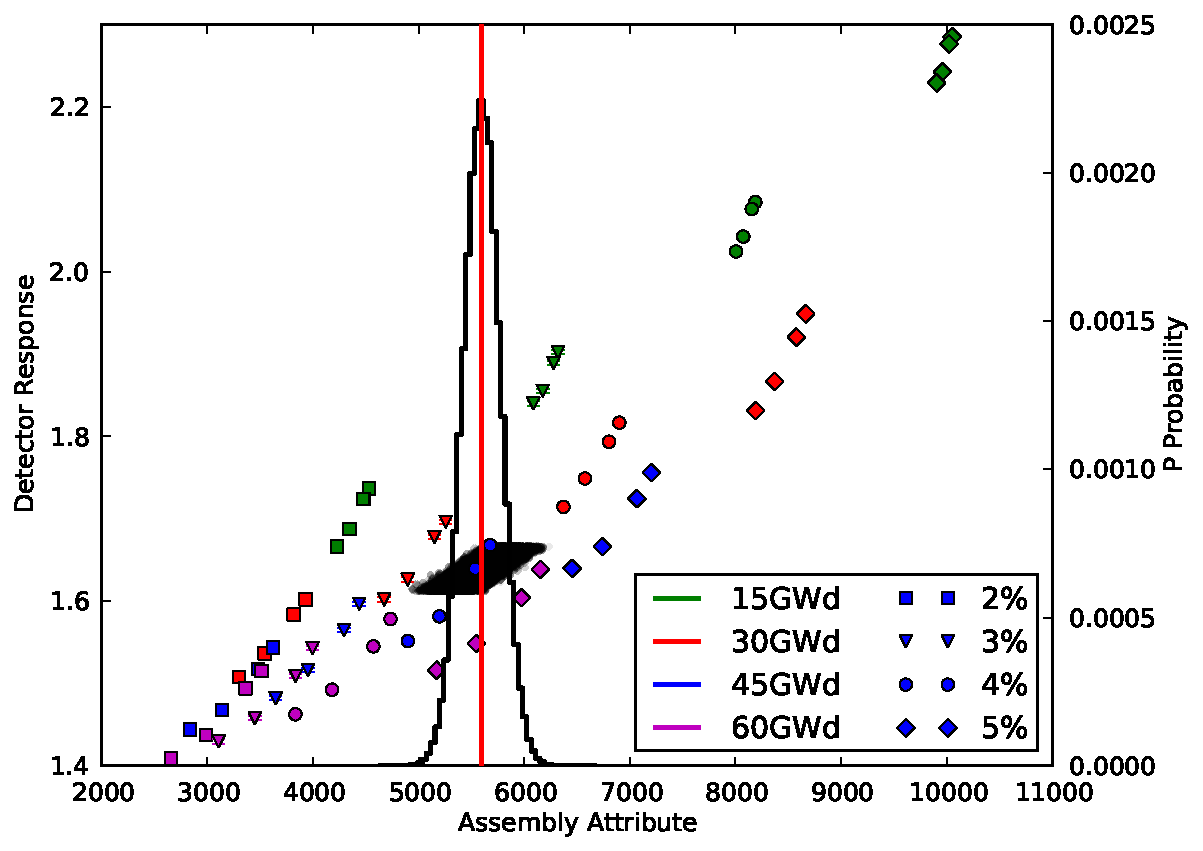
\includegraphics[width=0.45\textwidth, keepaspectratio]{Figures/CheckLimited.pdf} \label{fig:CheckLimited}}
    \caption{Results of estimating the assembly attribute measured by the PNAR-FC instrument without using the MCNPX simulation results for assembly models with \SI{45}{GWd/tU} burnup values.}
    \label{fig:Check}
\end{figure}

The second assessment we have attempted is to know how sensitive the Monte Carlo-based method is to a change in the uncertainty in the ``measured'' detector response.  Remember we have assumed an uncertainty of 1\%.  We have repeated the simulations, but with measured detector uncertainties of 1, 5, and 10\%.  The results are summarized in Table \ref{tab:CheckManyUncertainty} and shown graphically in Figure \ref{fig:CheckManyUncertainty}; Figure \ref{fig:CheckManyUncertaintyFull} shows the results when a full range of parameter values are used for sampling and Figure \ref{fig:CheckManyUncertaintyLimited} shows a limited range of sampling values.

\begin{table}[h!]\centering
    \begin{tabular}{@{}S@{}S@{}S}
        \toprule
        {Measured} & {\multirow{2}{*}{Full}} & {\multirow{2}{*}{Limited}} \\
        {Uncertainty} & & \\
        \midrule
        \SI{10}{\percent} & 5265(877) & 5619(260) \\
        \SI{5}{\percent}  & 5405(652) & 5615(255) \\
        \SI{1}{\percent}  & 5568(382) & 5597(176) \\
        \bottomrule
    \end{tabular}
    \caption{Results obtained by changing the ``measured'' uncertainty from 10\% to 1\% of the detector response.  The underlying data came from the PNAR-FC instrument.}
    \label{tab:CheckManyUncertainty}
\end{table}

\begin{figure}[hp!]\centering
    \subfloat[Full parameter range sampling.]{\includegraphics[width=0.45\textwidth, keepaspectratio]{Figures/CheckManyUncertaintyFull.pdf} \label{fig:CheckManyUncertaintyFull}} \qquad
    \subfloat[Limited parameter range sampling.]{\includegraphics[width=0.45\textwidth, keepaspectratio]{Figures/CheckManyUncertaintyLimited.pdf} \label{fig:CheckManyUncertaintyLimited}}
    \caption{Demonstration of the change in assembly attribute distribution with changing measured uncertainty.  The measured uncertainty shown is 10\%, 5\%, and 1\%; the 1\% uncertainty is the same as for the previous simulations.  The underlying data came from the PNAR-FC instrument.}
    \label{fig:CheckManyUncertainty}
\end{figure}
    
The results show that as the measured uncertainty increases, the uncertainty in the Monte Carlo results increase (as expected) but that the results are all within one standard deviation of each other.  This gives confidence that there is no bias introduced when the measured uncertainty increases.  Perhaps more interesting is that when independent information is known about the assembly parameters allowing a more limited range of sampling, the measured uncertainty is much less important.  Figure \ref{fig:CheckManyUncertaintyLimited} shows that the three simulations have nearly the same result---well within one standard deviation---and that the uncertainty in the assembly attribute is similar regardless of the measured uncertainty.

We now show another set of three simulations where we investigate the sensitivity of the estimated assembly attribute is to the number of Monte Carlo trials.  The results of these simulations are given in Table \ref{tab:CheckManyN} and shown in Figure \ref{fig:CheckManyN}.  The number of Monte Carlo trials for these simulations ranged from \num{1E2} to \num{1E6}.  

\begin{table}[h!]\centering
    \begin{tabular}{r@{}S@{}S}
        \toprule
        {$N$} & {Full} & {Limited} \\
        \midrule
        \num{1E2} & 5430(752) & 5612(283) \\
        \num{1E4} & 5405(645) & 5614(254) \\
        \num{1E6} & 5404(651) & 5616(255) \\
        \bottomrule
    \end{tabular}
    \caption{Results obtained by changing the number of Monte Carlo trials, $N$, from \num{1E2} to \num{1E6}.  The underlying data came from the PNAR-FC instrument.}
    \label{tab:CheckManyN}
\end{table}

\begin{figure}[hp!]\centering
    \subfloat[Full parameter range sampling.]{\includegraphics[width=0.45\textwidth, keepaspectratio]{Figures/CheckManyNFull.pdf} \label{fig:CheckManyNFull}} \qquad
    \subfloat[Limited parameter range sampling.]{\includegraphics[width=0.45\textwidth, keepaspectratio]{Figures/CheckManyNLimited.pdf} \label{fig:CheckManyNLimited}}
    \caption{Demonstration of the change in assembly attribute distribution with changing measured uncertainty.  The measured uncertainty shown is 10\%, 5\%, and 1\%; the 1\% uncertainty is the same as for the previous simulations.  The underlying data came from the PNAR-FC instrument.}
    \label{fig:CheckManyN}
\end{figure}

It is easy to see in Figure \ref{fig:CheckManyN} that changing the number of Monte Carlo Trials has big effect on the noise of an individual bin of assembly attribute, but that the distribution of the assembly attribute remains the same.  Table \ref{tab:CheckManyN} shows that the results of all the simulations are well within one standard deviation of each other indicating once again that no bias is introduced for a different number of Monte Carlo trials.  As before, we can see by comparing Figures \ref{fig:CheckManyNFull} and \ref{fig:CheckManyNLimited} that limiting the range of sampled parameter values greatly improves the estimate of the assembly attribute; in this case by reducing the noise of the individual assembly attribute bins in addition to reducing the uncertainty of the assembly attribute distribution.
    
In all of the simulations shown in this paper, we have chosen to estimate the assembly attribute for a reference assembly with parameters: \SI{45}{GWd/tU} burnup, \SI{4}{wt \% \isotope[235]{U}} initial enrichment, and \SI{5}{year} cooling time.  Our final validation assessment looks at the ability of the Monte Carlo-based method to accurately predict the assembly attribute for assemblies with parameters that differ from our reference assembly.  It would be impossible to explore all the possible combinations of assembly parameters in this paper so we have limited our assessment to four additional assemblies.  These four assemblies all have \SI{4}{wt \% \isotope[235]{U}} initial enrichment and \SI{5}{yr} cooling time; they differ in their burnup with a range of \SIrange{15}{60}{GWd/tU}.  

As with all of our simulations in this paper, we have done two simulations for each assembly; one with a full range of parameter values to sample, the other with a limited range of parameters.  The results of all the simulations are given in Table \ref{tab:AlternateAssemblies}; the results with the full range of parameter sampling are shown in Figure \ref{fig:AltFull} and the results with the limited range of parameter sampling are shown in Figure \ref{fig:AltLimited}.  These results again show the validity of the Monte Carlo-based method for estimating the assembly attribute.  With the exception of the assembly with \SI{15}{GWd/tU} burnup, all of the simulations utilizing the full range of parameter sampling fall within one standard deviation of the reference value; the assembly with \SI{15}{GWd/tU} is easily within two standard deviations.  All of the simulations utilizing a limited range of parameter sampling are well within the one standard deviation of the reference assembly.  Again we see the importance of using information on assembly parameters from independent measurements.

\begin{table}[h!]\centering
    \begin{tabular}{rc@{}S@{}S}
        \toprule
        Burnup & {Simulation} & {Full} & {Limited} \\
        \midrule
        15 & 8155 & 8407(215) & 8100(183) \\
        30 & 6803 & 6407(449) & 6778(192) \\
        45 & 5535 & 5567(386) & 5597(177) \\
        60 & 4571 & 4898(386) & 4789(170) \\
        \bottomrule
    \end{tabular}
    \caption{Estimated assembly attribute for four reference assemblies.  All assemblies have \SI{4}{wt \% \isotope[235]{U}} initial enrichment and \SI{5}{yr} cooling time; they differ in their burnup with a range of \SIrange{15}{60}{GWd/tU}. The underlying data came from the PNAR-FC instrument.}
    \label{tab:AlternateAssemblies}
\end{table}

\begin{figure}[hp]\centering
    \subfloat[\SI{15}{GWd/tU}]{\includegraphics[width=0.45\textwidth, keepaspectratio]{Figures/AlternateAssemblies/Burnup15Full.pdf} \label{fig:Alt15GWdFull}} \qquad
    \subfloat[\SI{30}{GWd/tU}]{\includegraphics[width=0.45\textwidth, keepaspectratio]{Figures/AlternateAssemblies/Burnup30Full.pdf} \label{fig:Alt30GWdFull}} \\
    \subfloat[\SI{45}{GWd/tU}]{\includegraphics[width=0.45\textwidth, keepaspectratio]{Figures/AlternateAssemblies/Burnup45Full.pdf} \label{fig:Alt45GWdFull}} \qquad
    \subfloat[\SI{60}{GWd/tU}]{\includegraphics[width=0.45\textwidth, keepaspectratio]{Figures/AlternateAssemblies/Burnup60Full.pdf} \label{fig:Alt60GWdFull}}
    \caption{Results from estimating the assembly assembly attribute for an assembly with \SI{4}{wt \% \isotope[235]{U}} initial enrichment and \SI{5}{yr} cooling time and a burnup of \SI{15}{GWd/tU} \subref{fig:Alt15GWdFull}, \SI{30}{GWd/tU} \subref{fig:Alt30GWdFull}, \SI{45}{GWd/tU} \subref{fig:Alt45GWdFull}, \SI{60}{GWd/tU} \subref{fig:Alt60GWdFull}.  The sampling range of parameters in the Monte Carlo estimation is the full range of possible assembly parameters.  The underlying data comes from the PNAR-FC instrument.}
    \label{fig:AltFull}
\end{figure}

\begin{figure}[hp]\centering
    \subfloat[\SI{15}{GWd/tU}]{\includegraphics[width=0.45\textwidth, keepaspectratio]{Figures/AlternateAssemblies/Burnup15Limited.pdf} \label{fig:Alt15GWdLimited}} \qquad
    \subfloat[\SI{30}{GWd/tU}]{\includegraphics[width=0.45\textwidth, keepaspectratio]{Figures/AlternateAssemblies/Burnup30Limited.pdf} \label{fig:Alt30GWdLimited}} \\
    \subfloat[\SI{45}{GWd/tU}]{\includegraphics[width=0.45\textwidth, keepaspectratio]{Figures/AlternateAssemblies/Burnup45Limited.pdf} \label{fig:Alt45GWdLimited}} \qquad
    \subfloat[\SI{60}{GWd/tU}]{\includegraphics[width=0.45\textwidth, keepaspectratio]{Figures/AlternateAssemblies/Burnup60Limited.pdf} \label{fig:Alt60GWdLimited}}
%   \caption{Limited  The underlying data came from the PNAR-FC instrument.}
\caption{Results from estimating the assembly assembly attribute for an assembly with \SI{4}{wt \% \isotope[235]{U}} initial enrichment and \SI{5}{yr} cooling time and a burnup of \SI{15}{GWd/tU} \subref{fig:Alt15GWdFull}, \SI{30}{GWd/tU} \subref{fig:Alt30GWdFull}, \SI{45}{GWd/tU} \subref{fig:Alt45GWdFull}, \SI{60}{GWd/tU} \subref{fig:Alt60GWdFull}.  The sampling range of parameters in the Monte Carlo estimation is: \SI{4.0(2)}{wt \% \isotope[235]{U}}, \SI{5(1)}{yr} with the burnup sampled from a gaussian centered at the burnup value (\SIlist[list-final-separator={, or }]{15; 30; 45; 60}{GWd/tU}) with a 5\% standard deviation.  The underlying data comes from the PNAR-FC instrument.}
    \label{fig:AltLimited}
\end{figure}

The fact that the estimate of the assembly attribute of the assembly with \SI{15}{GWD/tU} burnup falls slightly outside one standard deviation of the reference value is not too surprising.  Note that the estimate from the assembly with \SI{60}{GWd/tU} is almost outside one standard deviation.  Both of these assemblies lie on the edge of the mapped parameter space and we expect the quality of the mapping to be less certain on the edges of the parameter space.  Nevertheless, the Monte Carlo-based technique was able to accurately (within two standard deviations or better) estimate the assembly attribute even at the extremes of the parameter space.  
\section{Conclusions}\label{sec:Conclusions}
This paper introduced a Monte Carlo-based method of estimating attributes of spent fuel assemblies, such as the fissile content of the assembly.  The method utilizes results from MCNPX simulations of a variety of spent fuel assembly models and interpolates between these results to construct functions that map assembly parameters (e.g., burnup, initial enrichment, and cooling time) to either a detector response or an assembly attribute.  We have chosen to use radial basis functions to perform our interpolation since they can interpolate in many dimensions.  The use of the mapping functions is a method of emulating MCNPX simulations and reduces the computational expense by ten orders of magnitude.  

This analysis was developed to estimate the mean and distribution of values for a specific assembly attribute and is applicable to all of the fourteen NDA instruments we are currently investigating.  This Monte Carlo-based method is independent of the detector response and assembly attribute.  While all the results from the instruments shown in this paper detect neutrons in some fashion, the quantified assembly attributes include the fissile content of the assembly as well as the \isotope[239]{Pu} mass.

We have demonstrated this method for six different NDA instruments whose responses and assembly attributes were simulated for 64 different spent fuel assembly models.  For each instrument, we performed this Monte Carlo-based analysis and compared the result to one of the individually simulated spent fuel assembly model results.  Two simulations were performed, one using the full range of possible assembly parameter values and the another with a limited range of assembly parameter values.  In both cases, the estimated mean was well within two standard deviations of the original MCNPX simulation and for some instruments, within one standard deviation.

We have made a few additional simulations (in Section \ref{sec:Validation}) to assess the validity and sensitivity of this technique.  All of the simulations indicate that the Monte Carlo-based method is appropriate for estimating the assembly attribute of an unknown assembly, based upon a measured detector response.  One must be careful when estimating the assembly attribute for assemblies on the periphery of the mapped parameter space.

We would like to emphasize the importance of using independent measurements of the assembly parameters of burnup, initial enrichment, and cooling time.  When independent measurements of these parameters are used, the estimate of the assembly attribute is always better (i.e., a smaller uncertainty) compared to when independent measurements are not available.  In addition to reducing the uncertainty of the estimated assembly attribute, using independent measurements to estimate the assembly parameters reduces the number of Monte Carlo trials needed, improves the assembly attribute estimate at the periphery of the parameter space, and reduces the dependence on the measured detector response.

The Monte Carlo-based method introduced in this paper is a promising approach for estimating assembly attributes using emulated data based upon results from explicit simulation.  In creating the mapping functions we have assumed that the results from explicit MCNPX modeling had no uncertainty.  To accurately quantify the uncertainty in the estimated assembly attribute, the uncertainty in the simulations that provide the framework for the mapping functions must be propagated to the uncertainty in the distribution of the assembly attribute.  

We intend to use the Monte Carlo-based method to assist measuring the plutonium content in spent nuclear fuel assemblies as part of the NGSI effort.  A calibration is needed so that the modeled assemblies match the real-world assemblies.  A calibration of this sort would require an assembly with well known parameters.  The detector response from the NDA techniques would be calibrated to this known assembly and the modeled assemblies could alter the mapping of assembly attributes and detector responses to make the Monte Carlo-based estimate of the assembly attribute accurate to the specific system being measured.  One goal of such a calibration is to allow us to include an MCNPX model-error component of uncertainty, which is currently ignored.

Once the calibration has been performed measurements of the spent fuel assembly would be made with a variety of NDA techniques.  Inevitably, the assemblies measured would not have the same parameters as the assemblies which have been explicitly modeled.  The Monte Carlo-based method for estimating the assembly attribute would be used and the detector responses would be used as inputs to the method.  The estimated assembly attribute from the Monte Carlo-based method would be the best estimate based upon the measured detector response and the independent measurements of the assembly attributes.

\section{Acknowledgements}
This work was performed under the sponsorship of the Next Generation Safeguards Initiative.

The authors would like to thank the following individuals (in no particular order) Dr.~John Lestone at Los Alamos National Laboratory for his idea of using Monte Carlo techniques for this type of analysis.  Dr. Tom Burr at Los Alamos National Laboratory for his statistical help.  Dr.~Jesse Cheatham at Oak Ridge National Laboratory for his initial investigation into this domain.  Dr.~John Hendricks for his comments and suggestions on the Monte Carlo process.  

\bibliography{Bibliography}

\end{document}

